\subsection{Réseaux dans leurs contextes}
\begin{itemize}
\item réseau social : similitude entre amis (on voudrait mettre ces similitudes dans le réseau)
\item réseau d'affiliation - social 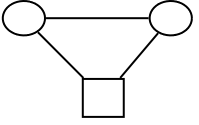
\includegraphics[scale=0.2]{images/21_Sim.png} <- explication d'une similitude \\
	- personnes \\
	- points d'intérêts 
\end{itemize}

\textbf{Idée générale}

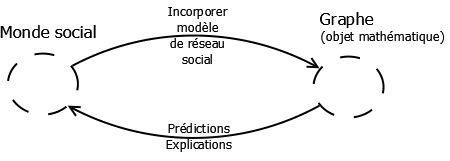
\includegraphics[scale=0.4]{images/21_IdeeGenerale.png}

\subsection{Exemples}
Il y a trois formes de fermeture
\begin{enumerate}
\item Fermeture triadique 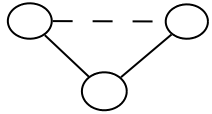
\includegraphics[scale=0.1]{images/21_FermetureTriadique.png}
\item Fermeture focale 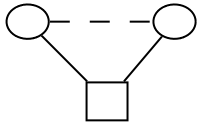
\includegraphics[scale=0.1]{images/21_FermetureFocale.png}
\item Fermeture d'adhésion 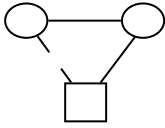
\includegraphics[scale=0.1]{images/21_FermetureAdhesion.png}
\end{enumerate}

\section{La formation des liens (selon les 3 approches)}
\begin{itemize}
\item On a des données réelles -> réseaux sociaux \\
		On a plus facilement un accès direct au graphes qu'avant.
\item mesurer empiriquement le taux de création des liens en fonction du nombres d'amis communs.
\end{itemize}

\subsection{Algorithme}
\begin{enumerate}
\item Capture à deux instants différents le réseau (appelons ces deux graphes (1) et (2))
\item Pour chaque entier "k" plus grand ou égal à 0 :
\begin{itemize}
	\item On identifie les paires de noeuds qui ont "k" amis en communs dans (1)
\end{itemize}
\item On regarde dans (2) si pour chaque paire un lien s'est formé
\end{enumerate}
=> On calcule T(k) = fraction des paires qui ont formé un lien

\subsection{Modèle pour expliquer ce résultat (fermeture triadique)}
Si on prend deux personnes : s'il y a 1 ami en commun, il y a une probabilité "p" qu'un lien se forme.\\
Quelle est la probabilité pour "k" amis en commun ?\\
=> On calcule la probabilité de "aucun lien se forme".

\paragraph*{}
La probabilité qu'aucun lien se forme quand il y a un ami en commun est de $(1-p)$.\\
On en déduit que pour "k" amis en commun, la probabilité est de $ (1-p)^{k}$\\
Dès lors, la probabilité qu'au moins 1 lien se forme pour k amis en commun est de $ 1-(1-p)^{k}$. C'est ce qui est égal à T(k).

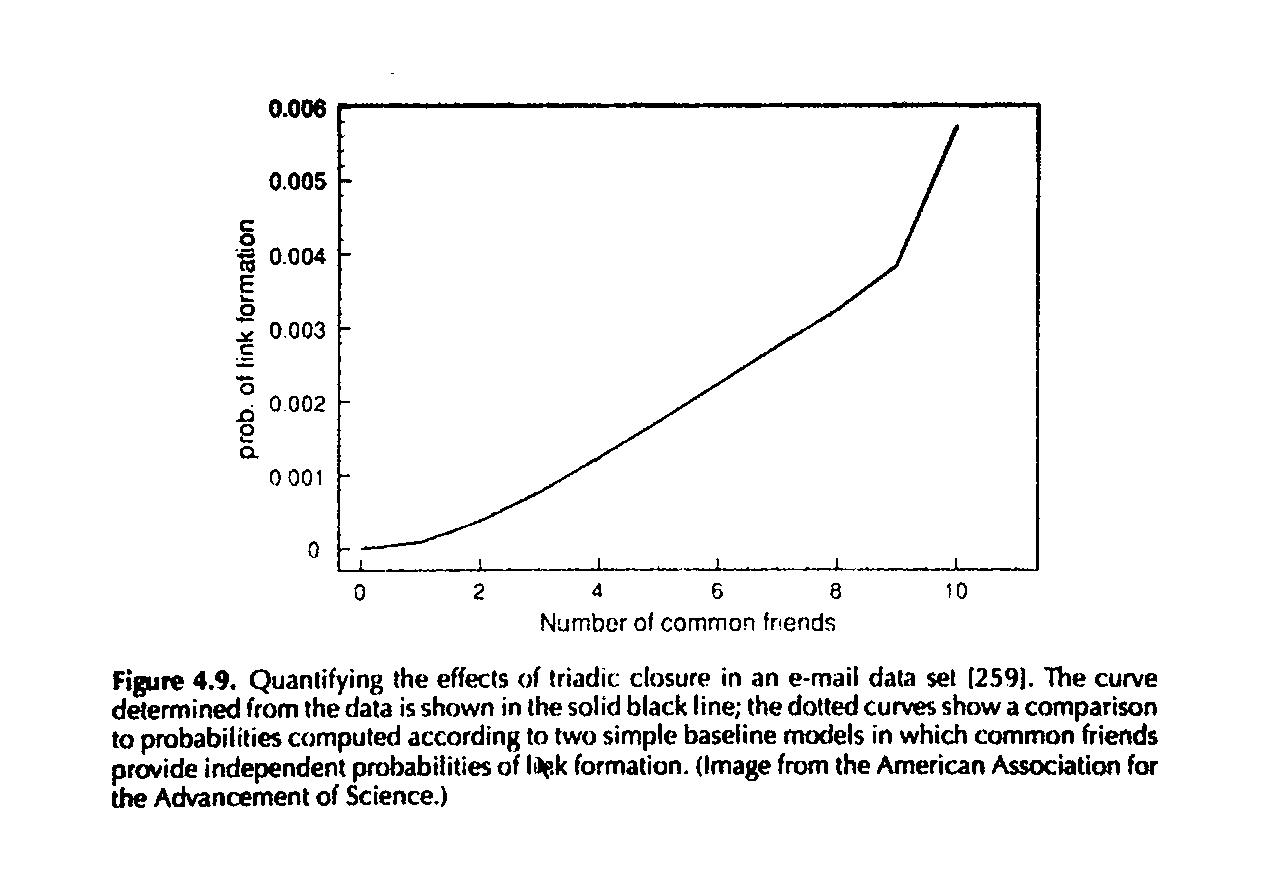
\includegraphics[width=\textwidth]{images/21_emailFriends.jpg}

On voit sur la figure 4.9 (fermeture triadique) que la probabilité qu'un lien se forme augmente exponentiellement avec le nombre d'amis en commun.

\paragraph{Attention !}
Le comportement et donc les calculs sont différents pour la fermeture focale et d'adhésion !

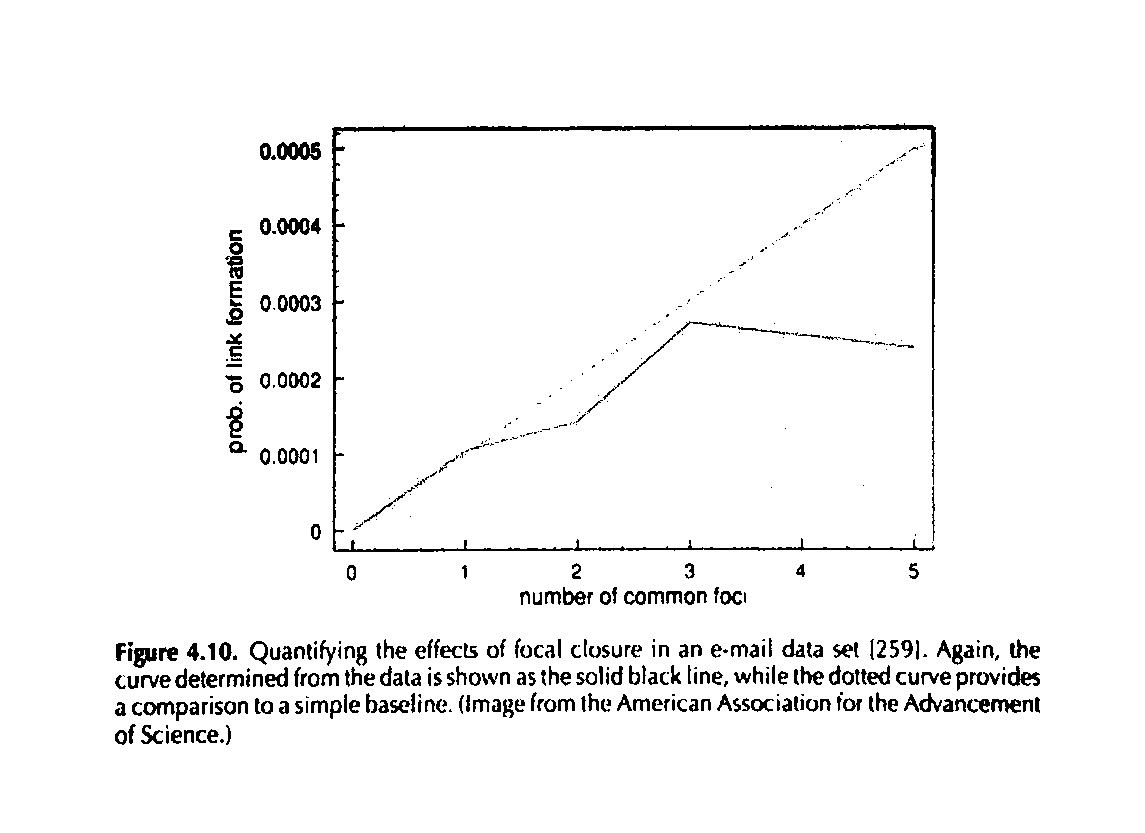
\includegraphics[width=\textwidth]{images/21_pointsCommuns.jpg}

La figure 4.10 (fermeture focale) nous montre que dans le cas où l'on considère le nombre d'intérêts en commun (ici, des cours), on arrive à un certains moment à saturation. Augmenter le nombre de points d'intérêts communs n'augmente plus la probabilité de création d'un lien à partir d'un certain point (ici 3 cours en communs).

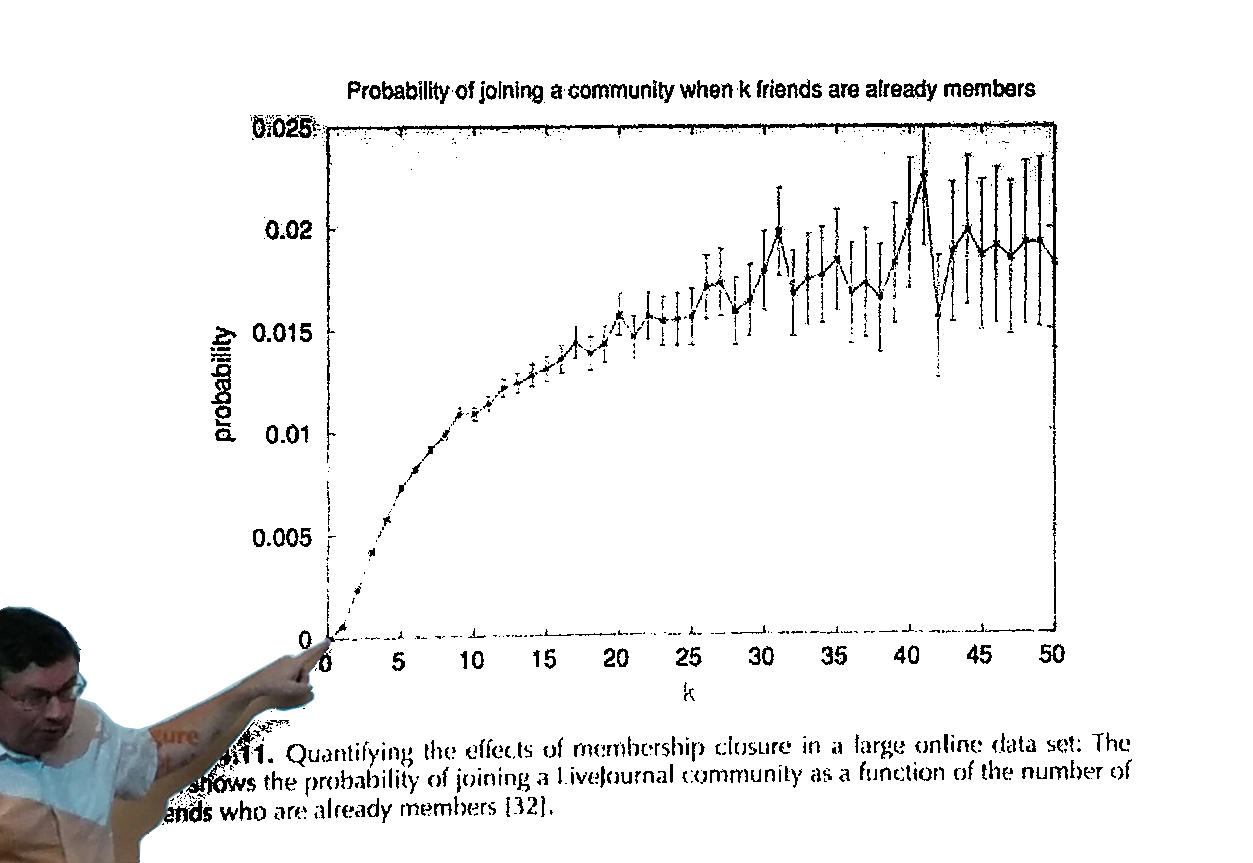
\includegraphics[width=\textwidth]{images/21_community.jpg}

Enfin, la figure 4.11 (fermeture d'adhésion) présente aussi un saturation à partir d'un certains nombre d'amis qui ont le même point d'intérêt.

\section{Quantifier les rôles relatifs de sélection d'influence sociale}
Les mécanismes de similitude :
\begin{itemize}
\item La sélection (intérieur, c'est nous qui faisons le choix)
\item L'influence sociale (extérieur, c'est les autres qui nous influencent) 
\end{itemize}
\subsection{Comment quantifier cela ?}
\paragraph*{Par exemple wikipédia}
Il peut exister une similitude de comportement entre rédacteurs. Par exemple les articles sur lesquels ils travaillent.\\
Raisonnement :
\begin{itemize}
\item On a des rédacteurs
\item Un lien entre deux rédacteurs : ils communiquent par la "Talk page" (chaque article a une "Talk page"). Autrement dit, si un rédacteur B communique sur la page de A, alors il y a un lien.
\item Les "points d'intérêts" ici sont les articles.
\item Quantification de la similitude = $\displaystyle\frac{\mbox{nombre d'articles rédigés par A ET B}}{\mbox{nombre d'articles rédigés par A OU B}}$\\
Notons dès lors que la similitude ne peut pas être plus petit que 0 ni plus grand que 1. $0 \leq sim \leq 1$
\item La rupture se fait quand le lien est créé. %schéma
\item On compare la similitude avant et après cette rupture (figure 4.13). C'est surtout la sélection qui joue avant, et l'influence sociale rentre en jeu après.
\end{itemize}

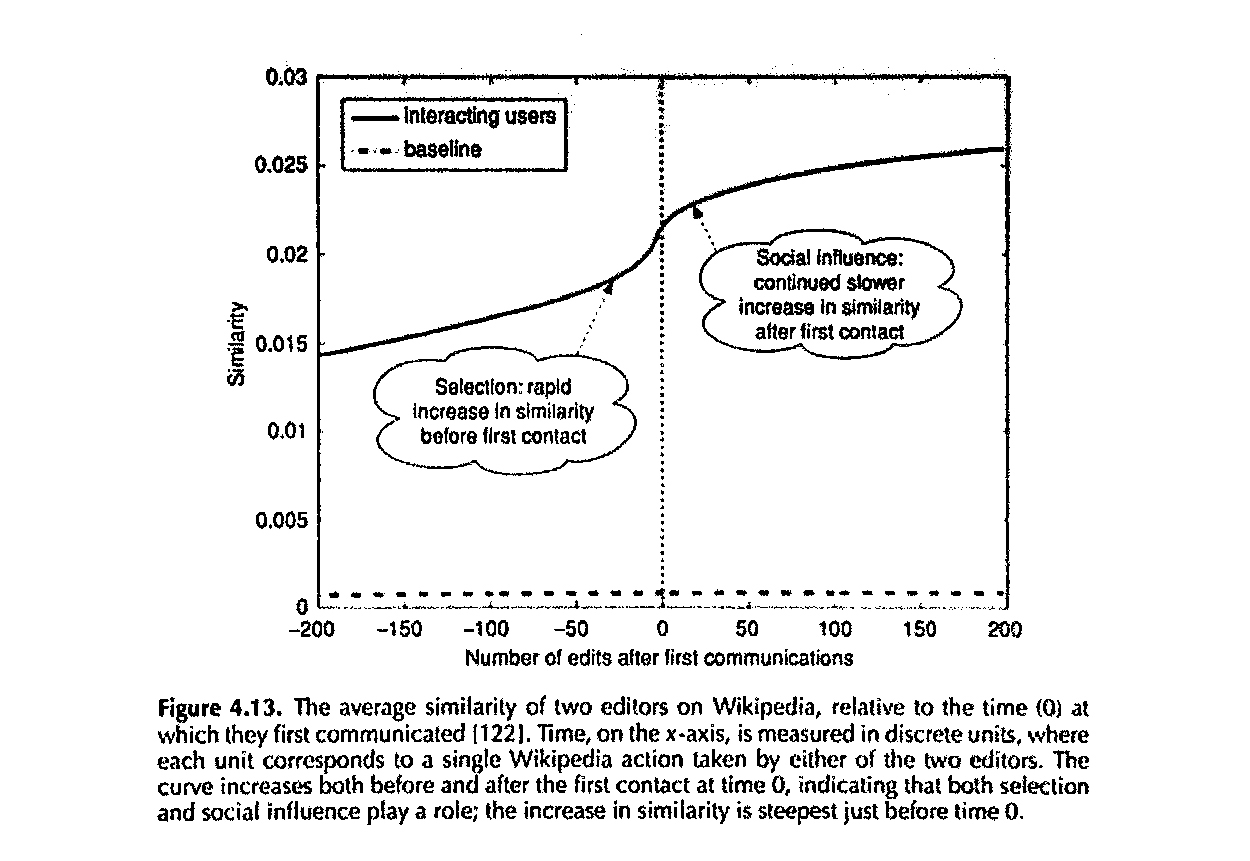
\includegraphics[width=\textwidth]{images/21_wikipedia.jpg}